

%******************************************************************************
% *filename:		systemDesign.tex
% *author:  		synckey
% *version: 		v1.0
% *datetime:		2011-06-23 13:18
% *description:
% *****************************************************************************/
\documentclass[12pt, a4paper, titlepage]{article}
\usepackage{titletoc}
\usepackage{fontspec}
\usepackage{graphicx}
\usepackage{array}
\usepackage{longtable}
\usepackage{paralist}
\usepackage{float,longtable}
\usepackage{enumerate}
\usepackage{xcolor,listings}
\usepackage{booktabs, multirow}
\usepackage[pagestyles]{titlesec}
\usepackage{xeCJK}
\lstset{
	numbers=left,%行号
	framexleftmargin = 2em,%背景框
	frame = none,
	backgroundcolor = \color[RGB]{245, 245,244},
	keywordstyle = \bf\color{blue},
	identifierstyle = \bf,
	numberstyle=\color[RGB]{0,192,192},
	commentstyle=\it\color[RGB]{0,96,96},
	stringstyle=\rmfamily\slshape\color[RGB]{128,0,0},
	showstringspaces=false
}


\newcommand{\codebox}[3]
{
\begin{center}
\fbox{
	\begin{minipage}[b]{130mm}
		#1\\
		#2
		\begin{flushright}
		返回值:#3
		\end{flushright}
	\end{minipage}
}
\end{center}
}


\titlecontents{section}[4em]{\small}{\contentslabel{3.3em}}{}
	{\titlerule*[0.5pc]{$\cdot$}\contentspage}
\titlecontents{subsection}[7em]{\small}{\contentslabel{3.3em}}{}
	{\titlerule*[0.5pc]{$\cdot$}\contentspage}
\titlecontents{subsubsection}[7em]{\small}{\contentslabel{3.3em}}{}
	{\titlerule*[0.5pc]{$\cdot$}\contentspage}
\renewcommand{\today}{\number\year-\number\month-\number\day}
\setmainfont[BoldFont=SimHei]{SimSun}
\setmonofont{SimSun}
\XeTeXlinebreaklocale"zh"
\title{DNS缓存系统系统设计说明书}
\author{v1.0}
\newpagestyle{mypagestyle}{
	\sethead{\sectiontitle}{}{$\cdot$~\thepage~$\cdot$
	}
	\setheadrule{1pt}
	\setfoot{}{}{\headrule}
}
\newpagestyle{myempty}{
	\sethead{\sectiontitle}{}{}
	\setheadrule{1pt}
	\setfoot{}{}{\headrule}
}
\renewcommand{\contentsname}{目\quad 录}
\renewcommand{\figurename}{图}
\renewcommand{\tablename}{表}
\renewcommand{\refname}{参考文献}
\pagestyle{mypagestyle}
\makeatletter
\let\@afterindentfalse\@afterindenttrue
\@afterindenttrue
\makeatother
\setlength{\parindent}{2em}%中文缩进两个汉字位
\linespread{1.25}
\usepackage[pagebackref,colorlinks, linkcolor = blue , urlcolor = blue]{hyperref}
\newcommand{\tabincell}[2]{\begin{tabular}{@{}#1@{}}#2\end{tabular}}

\begin{document}
\maketitle
\begin{table}[H]
\centering
\centering\Large\textbf{修改记录}\\[15pt]
\begin{tabular}{|p{2em}|c|p{9em}|c|}
\hline
\centering\textbf{No} &  \tabincell{c}{ \textbf{修改后} \\ \textbf{版本号}} 
& \centering \textbf{修改内容简介}&\textbf{修改日期 } \\
\hline
\centering 1 & v1.0 & 第一版 &2011.06.23\\
\hline&&&\\\hline&&&\\\hline&&&\\\hline&&&\\\hline
\end{tabular}
\end{table}
\thispagestyle{myempty}
\newpage
\pagenumbering{Roman}
\tableofcontents
\newpage
\pagenumbering{arabic}

\section{引言}

\subsection{编写目的}
	\indent
	本文档详细介绍了DNS缓存系统的系统设计,描述出一个具体的产品
	设计模型,为开发及测试人员提供下步工作的依据。

\subsection{背景}
	\indent
	本系统的开发满足需求设计中对本系统的要求。它提供DNS缓存服务,网络中的主
	机可以一次向本系统提出多个DNS请求,系统以尽快的速度予以响应。这样
	就避免了客户端频繁的DNS请求,加快了客户端的速度。另外,客户在一次请求中
	可以请求多个域名。本系统可以同时为多个客户端服务,采用多线程的方式来加快
	处理速度,初步设计为可以承受5000reqs/s的工作负担。采用比LRU效率更高的LIRS\cite{LIRS}
	技术来管理本地的缓存,可以提高系统的缓存命中率,减小了响应时间。


\section{总体设计}
\subsection{软件体系结构}

\begin{figure}[H]
\centering
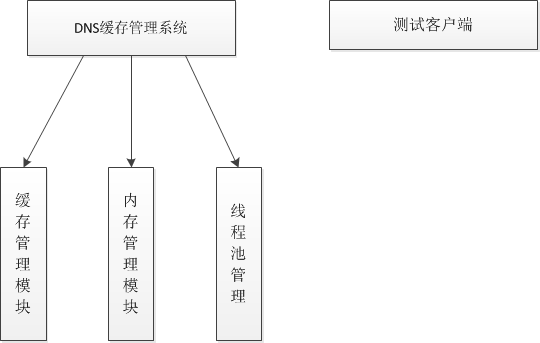
\includegraphics[keepaspectratio, scale=0.9]{pitures/zixitongcengcitu.png}
\caption{DNS缓存系统子系统层次图}
\end{figure}
\indent DNS缓存系统是一个DNS的一个高速缓存服务器,提供DNS缓存服务。传统的DNS服务
	器一次只能查询一个域名,而且响应速度慢。本系统将为客户端代理DNS请求
	,把DNS查询结果返回给客户端,并且把结果缓存在本地。当客户下一次请求同样
	的域名时,就可以在本地的缓存中查找,如果缓存中存在未被替换的结果,则返回
	该结果;否则,系统重新请求DNS服务器,并将DNS服务器返回结果存入缓存
	中。客户可以在一次请求中查询多个域名的IP地址,本系统予以响应。我们把整
	个系统分为三个大的模块:
	\begin{compactitem}
	\item{\textbf{缓存管理模块:} 把从DNS处获得的IP地址在本地缓存。域名使用
	字典树\cite{IDAT}在本地组织,从而加快对域名的检索速度。在缓存区满了以后,采用比传统
	LRU算法效率更高的LIRS\cite{LIRS}算法,进行缓冲区的更新。}
	\item{\textbf{内存管理模块:}为了加快系统的响应速度,减少动态申请内存带
	来的时间损耗,为请求报文预分配一块内存区域,当客户有连接时,从用户报文的
	前四个字节中获取整个报文的长度,然后从内存管理模块中申请(不是动态申请)
	响应长度的内存区域。这一块内存还将被用于构建返回报文。}
	\item{\textbf{线程池管理模块:}为了减少创建和销毁线程所带来的系统开销,
	在系统中采用线程池技术。在系统启动时,创建一定数目的线程。主线程负责接受
	用户的请求,然后调用线程池中的线程为客户服务。线程池管理模块负责线程的创
	建,申请和回收。}
	\item{\textbf{测试客户端:}用于测试本DNS缓存系统是否正确工作,同时也测试它
	的并发性能。}
	\end{compactitem}
\subsection{运行系统}
\subsubsection{运行体系图}
\begin{figure}[H]
\centering
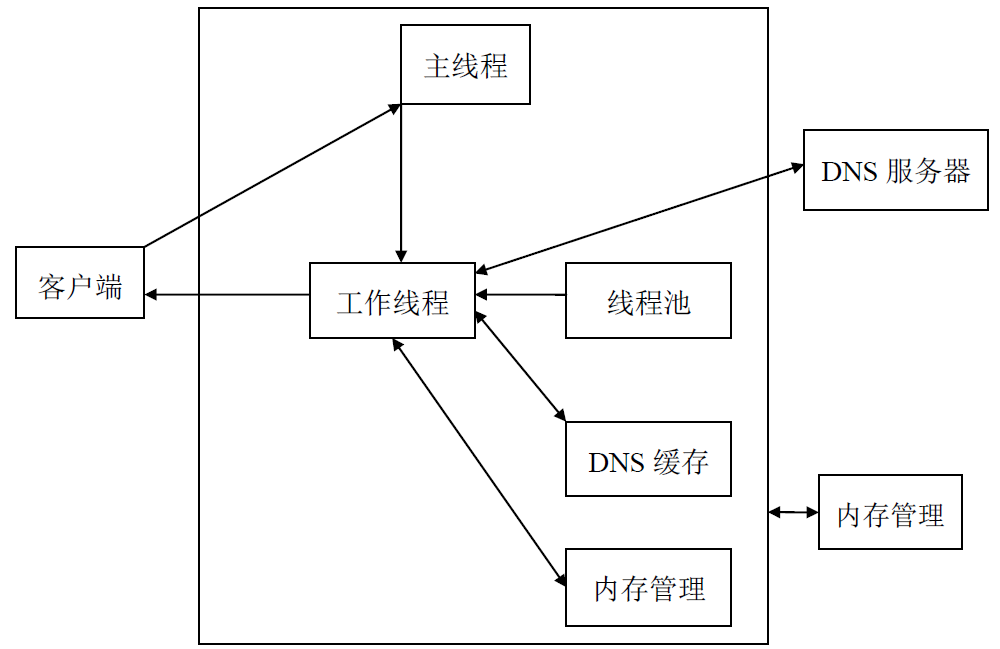
\includegraphics[keepaspectratio, scale=0.5]{pitures/xitongyunxing.png}
\caption{DNS缓存系统子系统层次图}
\end{figure}
\subsubsection{程序/模块对应表}
\begin{figure}[H]
\centering
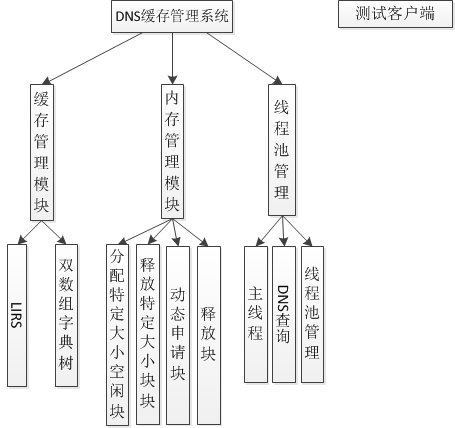
\includegraphics[keepaspectratio, scale=1]{pitures/struct.png}
\caption{程序/模块对应表}
\end{figure}


\subsection{系统物理结构}
\begin{figure}[H]
\centering
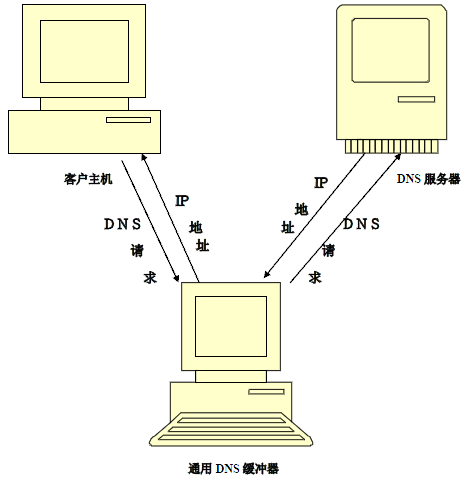
\includegraphics[keepaspectratio, scale=0.7]{pitures/xitongwulijiegou.png}
\caption{系统物理结构图}
\end{figure}

\section{系统环境}
\subsection{开发环境}
\begin{longtable}{%
@{\extracolsep{\fill}}>{\tt}ll@{}}
\toprule[1pt]
\multicolumn{1}{c}{环境}&
\multicolumn{1}{c}{工具}\\\midrule
操作系统	&	ubuntu11.04 x86\_64 \\
内核版本	&	2.6.38-8\\
编译器		&	gcc 4.5.2 \\

\bottomrule[1pt]\\[2pt]
\caption{开发环境}
\end{longtable}

%
%
%/******************************************************************************
% *filename:		shejisilu.tex
% *author:  		synckey
% *version: 		v1.0
% *datetime:		2011-06-24 14:21:17
% *description:
% *****************************************************************************/
\section{设计思路及折衷} 
\subsection{TCP OR UDP?}
由于可以在一个请求中接受多个域名的查询,所以数据包可能会非常大。UDP缺乏流控制和
错误控制,在数据量比较小的时候使用UDP非常合适。我们一个请求和应答的数据包可
能达到几十K,考虑到客户端的网络流量,如果使用UDP,肯定会发生错误或丢包,在应用程
序中处理错误和重传会造成资源浪费,加重服务器的负担,也会造成网络的拥堵,同时也加
大了客户的响应时间。
\par{而在数据量比较小的时候,使用UDP就非常合适。所以我们初步设计为提供两个服务器
,一个UDP服务器,和一个TCP服务器。客户端根据它的报文大小来选择使用UDP还是TCP。}
\subsection{为什么是LIRS而不是LRU?}
根据资料显示,LIRS的效率比LRU高,但是实现的代价比LRU高不了多少,所以使用LIRS。
\subsection{为什么是字典树,而不使用HASH函数?} 
采用字典树与HASH函数相比,有以下几点优势:
\begin{asparaenum}[1.]
\item{可以利用字符串的公共前缀来节约存储空间。} 
\item{查找效率比HASH高\cite{DATA}}
\item{HASH可能产生碰撞} 
\end{asparaenum}
\subsection{为什么使用两个双数组字典树?}
字典树的查询效率非常高,但是动态构造构造的过程非常慢,需要做大量的内存拷贝。在设计中使用
两个双数组字典树。把访问频度最高的几百万(可配置的数目)个域名存放在文件中,在系
统启动时,从文件中读入域名信息,用于构造主字典树(在已知大小时,字典树构造速度非常
快,因为不需要内存的动态分配和拷贝操作)。在查询域名时,首先从主字典树中查询,如
果未命中,就把相应域名加入副字典树中(副字典树比较小,动态构造小的字典树代价很低)。
这种方式,既保留了字典树的较高的查询速率,又避免了动态构造很大的字典树带来的开销
。

%
%/*********************************  END OF section{设计思路及折衷}  *********************************/





%/******************************************************************************
% *filename:		mokuaisheji.tex
% *author:  		synckey
% *version: 		v1.0
% *datetime:		2011-06-24 08:42:26
% *description:		模块设计
% *****************************************************************************/
\section{模块设计}
\subsection{线程池设计} 
在系统开始运行时创建MAXTHREAD个线程,放入线程池中。主线程创建监听套接字,开启服
务。每个线程各自调用accept,采用互斥锁来保证在每一个时刻只有一个线程调用accept。
每个线程在accept后为客户端服务。
\par{由于TCP内部为监听套接字维护两个队列:a.已完成队列,b.未
完成队列。所以在主线程睡眠期间,新的客户连接会使这两个队列充满(两个队列之和不超
过在listen时指定的backlog),而在这两个队列满了之后当一个客户的SYN到达时,TCP就
忽略该分节,也就时说,并不返回RST。这样做是因为:这种情况是暂时的,客户将重发SYN
,期望在不久就能在这些队列中找到可用空间\cite{unpv1}。 所以当这两个队列充满以后
,客户只是重发SYN ,而服务器不会接受客户端创建更多的连接。}
\begin{figure}[H]
\centering
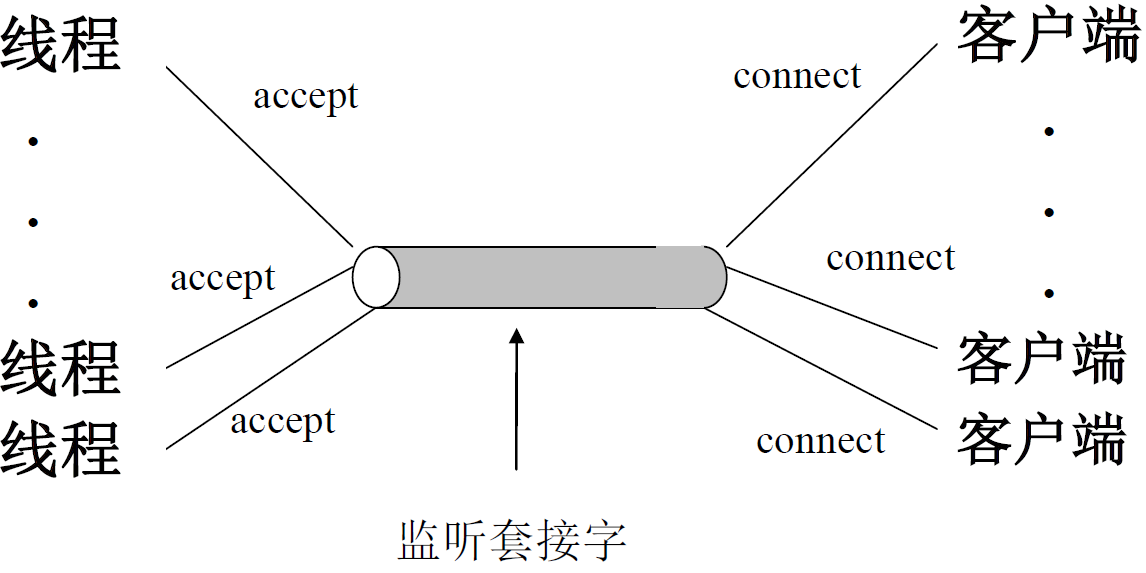
\includegraphics[keepaspectratio, scale=0.4]{pitures/xianchengmoxing.png}
\caption{多线程模型} 
\end{figure}
\subsection{工作线程设计}

线程池中的工作线程首先调用connect,接受一个客户端的连接,然后从报文的前4个字节中
获取报文的长度,从内存管理模块申请响应大小的内存,用于存放请求报文。
在收到请求后,逐次扫描每个域名。获得域名后,首先在本地的缓存中查找域名对应的IP,
如果有记录,就把IP地址填写到返回报文中,如果没有记录,则填入127.0.0.1,表明本地
没有缓存,将会进行DNS查询,结果在第二个报文中返回。然后把这个域名相应的序号和域
名填入到下图所示的链表中。

\begin{figure}[H]
\centering
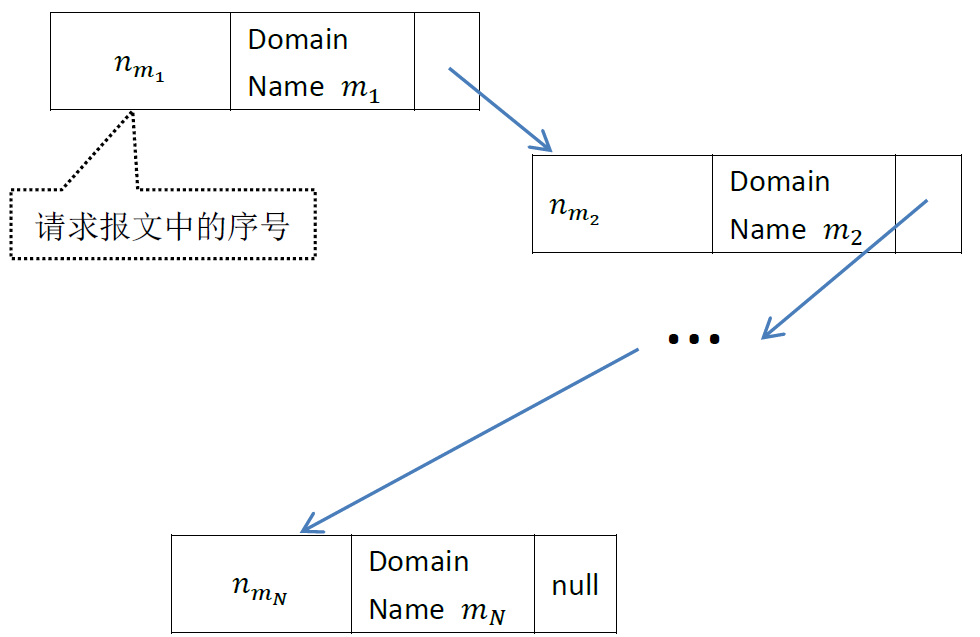
\includegraphics[keepaspectratio, scale=0.5]{pitures/response2_dns_list.png}
\caption{本地缓存未命中的域名构成的链表} 
\end{figure}

\par{工作线程在把请求报文遍历完毕后,就把第一次返回报文发送
给客户端,同时也把所有本地没有缓存的域名构造成了一个链表。如果链表为空,说明请求
的域名在本地都有缓存,任务完毕,关闭连接。否则,根据链表中的数目,申请用于构造第
二次返回报文的内存空间。对链表进行遍历,对链表中的每个域名调用一个DNS查询线程进行
DNS查询,在最后一个DNS查询完成后,把第二个报文发送给客户端,关闭连接。}

\begin{figure}[H]
\centering
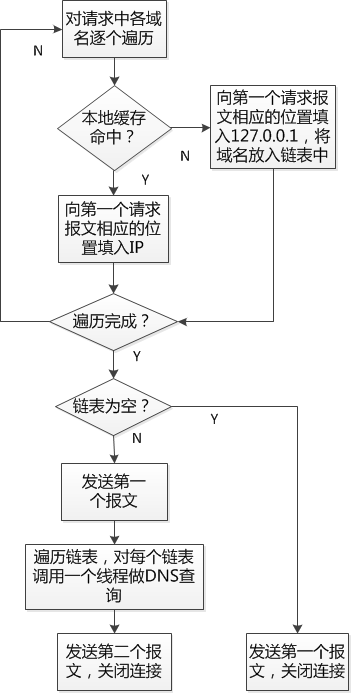
\includegraphics[keepaspectratio, scale=1]{pitures/xianchengliuchengtu.png}
\caption{线程工作流程图} 
\end{figure}


%%%%%%%%%%%%%%%%%%%%%%%%%%%%%%%%%%%%%%%%%%%%%%%%%
%                                               %
%filename	mm.tex				%
%author		wakemecn			%
%date		6/23/2011			%
%                                               %
%%%%%%%%%%%%%%%%%%%%%%%%%%%%%%%%%%%%%%%%%%%%%%%%%

%\documentclass{article}
%\usepackage{xeCJK}
%\setmainfont[BoldFont=SimHei]{SimSun%}
%\setmonofont{SimSun}
%\XeTeXlinebreaklocale"zh"
%\begin{document}
\subsection{内存管理模块}
		模块从系统预先申请256B,512B,1KB,2KB,$\ldots$,$2^n$KB等2幂次大小的块
		各若干。通过mem\_chunk结构维护特定大小的内存块大小的幂级,预分配的数目,
		已被使用的块链表和空闲的块链表。指针数组维护所有大小块的mem\_chuck结构
		指针。当申请使用M KB($2^m < M < 2^n$)空间时,若$2^n$KB大小块仍有空
		闲块,则将其分配,并将该块移动至已使用块链表中;若上述大小的块不存
		在空闲块或者不存在该大小的块,则模块动态申请若干数目该大小块的内存区域,
		分配内存。当释放某大小块时,若检测到释放的块位于模块动态申请的内存中
		时,则释放该内存。
\begin{figure}[H]
\centering
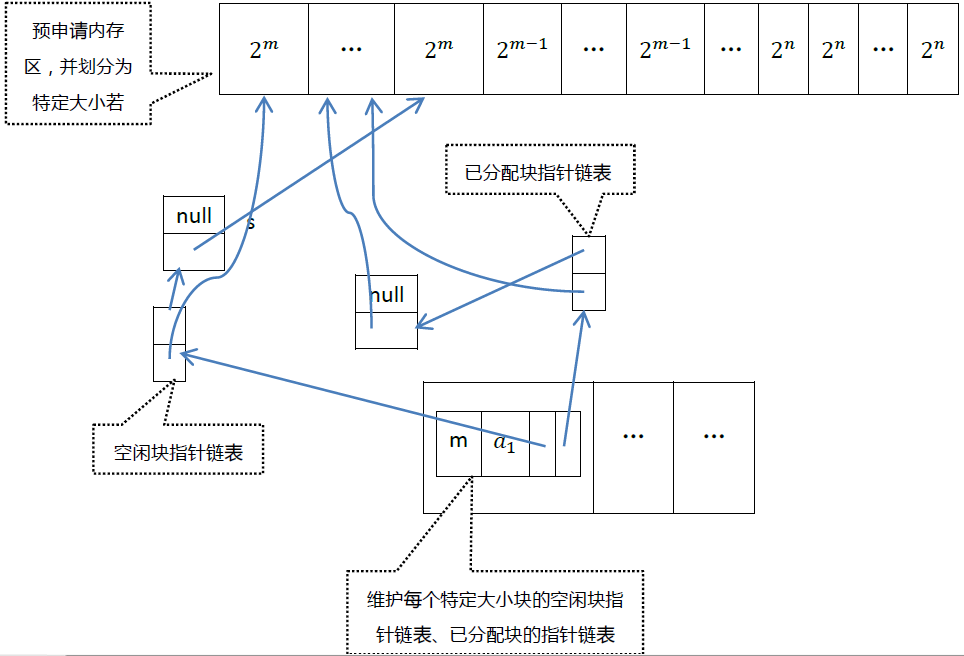
\includegraphics[keepaspectratio,scale=0.5]{pitures/mm.png}
\caption{内存管理示意图}
\end{figure}


%%%%%%%%%%%%%%%%	end of mm.tex    %%%%%%%%%%%%%%%


\subsection{缓存管理模块} 
%缓存管理模块由 DATrie 和 LIRS 栈驱动.
\textbf{定义1:}双数组Trie(Double-Array  Trie,DATrie)是 trie 树的一个简单而有效的实现,
由两整数数组构成,一个是 base[],另一个是check[]。check[base[s] + c] = s base[s]
+ c = t.
\par{对域名集合的索引是有两个双数组字典(Double-Array  Trie,DATrie)驱动的。其中
	一个 DATrie较大,存放所有已知域名集合,是静态的;另一个DATrie 较小,实际应用中作为较大的
	DATrie的补充,是动态变化的。每当动态DATrie 中记录达到一定数目时,就会离线补充静态DATrie
	中,失效域名从静态DATrie 中剔除。当有请求查询缓存是首先访问静态的DATrie,若没有命
	中则访问动态DATrie,当两者均未命中时选择向动态 DATrie中插入记录。 
}
\par{ 静态DATrie 由离线生成,并且不断从动态 DATrie 中学习补充。 }
\par{ 域名索引不仅是对缓存内容索引,由于DATrie 查询字符串速度快,但插入或删除效率较低因此采用上
	述两个DATrie结合的缓存方法。 }
\par{ 定义2:最短最近使用间隔算法(Low  Inter-Reference  Recency  Set,LIRS):LIRS算法是一中基于LRU算法
	弱点而改进的算法,使用页面的最近实用间隔(Inter-Reference Recency,IRR)来决定要替
	换的页面。IRR 用来表示一个页面的最近两次访问的间隔中的其他无重复页面的个数。LIRS 用来
	表示一个页面的最近两次访问的间隔中的其它无重复页面的个数。 LIRS还定义了一中不同的最
	近访问时间R(Recency,R ),R用来表示一个页面的最近访问至当前访问之间的其它无重复页面的个数。 }
\begin{figure}[H]
\centering
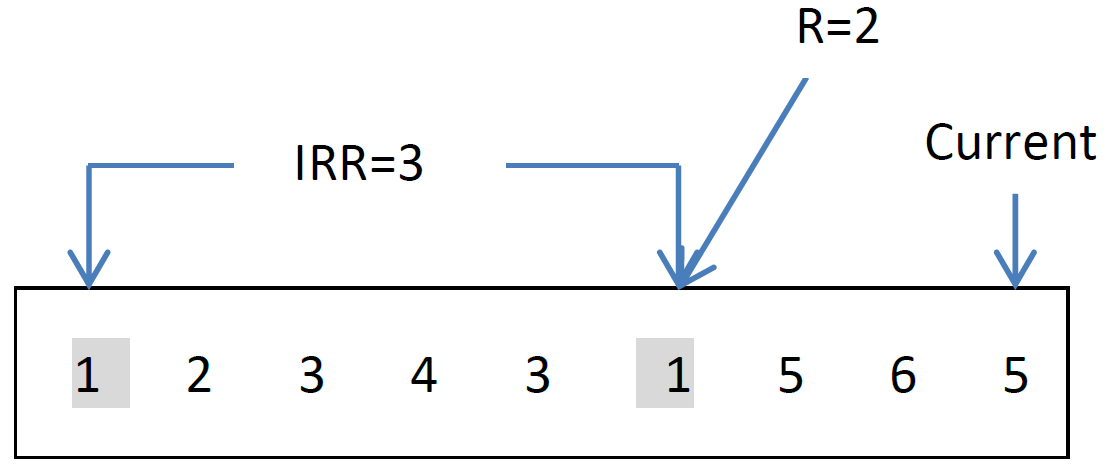
\includegraphics[keepaspectratio, scale=0.4]{pitures/irr.png}
\caption{LIRS算法的IRR和R的示意} 
\end{figure}

\begin{figure}[H]
\centering
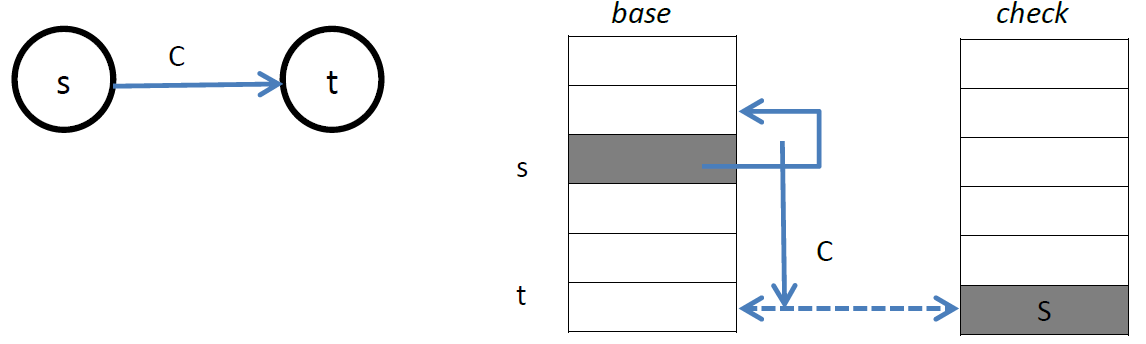
\includegraphics[keepaspectratio, scale=0.4]{pitures/aaa.png}
\caption{} 
\end{figure}

\begin{figure}[H]
\centering
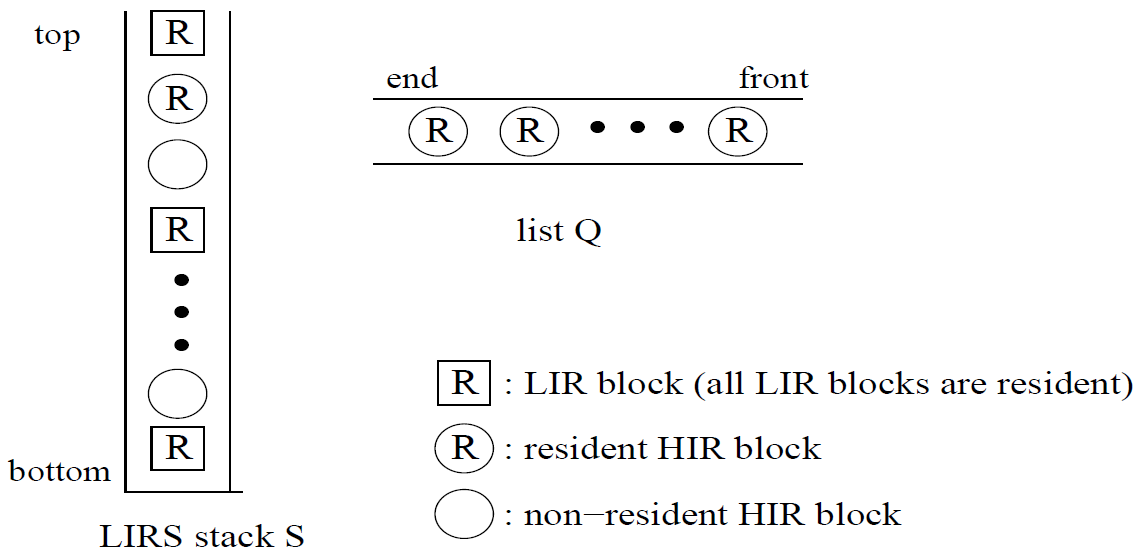
\includegraphics[keepaspectratio, scale=0.4]{pitures/lirsstack.png}
\caption{ DATrie 的状态转换示意,base[s]+c=t, check[t]=s } 
\end{figure}


%/*********************************  END OF mokuaisheji.tex  *********************************/




%
%
%/******************************************************************************
% *filename:		tongxinxieyi.tex
% *author:  		synckey
% *version: 		v1.0
% *datetime:		2011-06-24 11:25:45
% *description:		通信协议
% *****************************************************************************/
%
\section{通信协议}
\subsection{请求报文}
\begin{figure}[H]
\centering
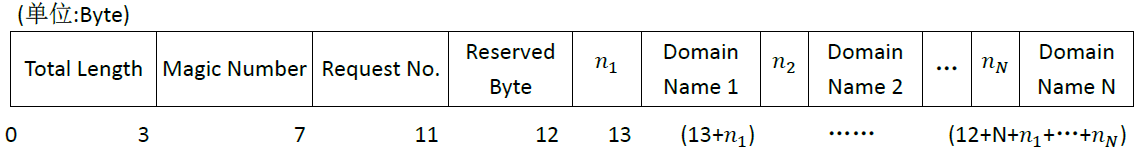
\includegraphics[keepaspectratio, scale=0.4]{pitures/request.png}
\caption{请求报文格式}
\end{figure}
	\begin{asparaitem}
		\item{报文总长度(Total Length)字段:占4字节。用来指定请求报文的总长度。}
		\item{魔数(Magic Number)字段:占4字节。用来区分UDP有效报文和垃圾报文。}
		\item{请求序列号(Request No.)字段:占4字节。用于标示同一台主机向系统请求DNS解析的请求编号。}
		\item{保留字节(Reserved Byte):占1字节。用于返回报文的错误控制、返回顺序等扩展。}
		\item{域名(Domain Name)字段:不定长字节数。给出要解析的具体域名。每个域名必须以 0 结尾。}
	\end{asparaitem}

\subsection{返回报文1}
\begin{figure}[H]
\centering
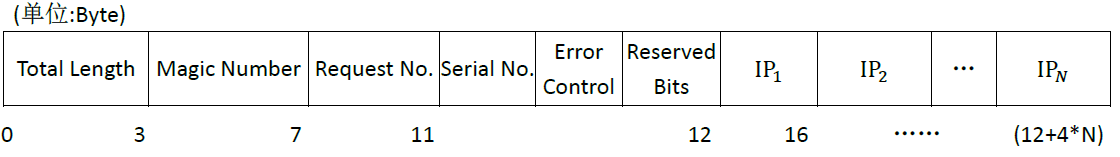
\includegraphics[keepaspectratio,scale=0.4]{pitures/response1.png}
\caption{返回报文1}
\end{figure}
	\begin{asparaitem}
		\item{报文总长度(Total Length)字段:占4字节。用来指定返回报文的总长度。}
		\item{魔数(Magic Number)字段:占4字节。用来区分UDP有效报文和垃圾报文。}
		\item{请求序列号(Request No.)字段:占4字节。用于标示同一台主机向系统请求DNS解析的请求编号。}
		\item{序列号(Serial No.)字段:占1比特。0表示第一次向特定请求返回报文。}
		\item{错误控制(Request No.)字段:占1比特。用于标示后续字节中存在域名解析失败的情况, 0表示
		有错,1表示没有错误。}
		\item{保留字位(Reserved Bits):占6比特。用于返回报文将来可能需要的其他扩展。}
		\item{网际协议地址(IP)字段:占4字节。用于给出请求报文中相应域名的对应IP地址,或者相应的错误代码。}
	\end{asparaitem}

\subsection{返回报文2}
\begin{figure}[H]
\centering
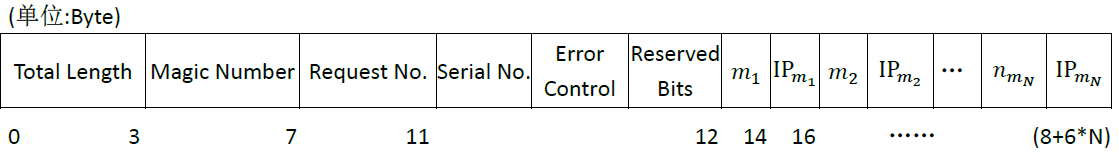
\includegraphics[keepaspectratio,scale=0.4]{pitures/response2.png}
\caption{返回报文2}
\end{figure}
	\begin{asparaitem}
		\item{报文总长度(Total Length)字段:占4字节。用来指定返回报文的总长度。}
		\item{魔数(Magic Number)字段:占4字节。用来区分UDP有效报文和垃圾报文。}
		\item{请求序列号(Request No.)字段:占4字节。用于标示同一台主机向系统请求DNS解析的请求编号。}
		\item{序列号(Serial No.)字段:占1比特。1表示第二次向特定请求返回报文。}
		\item{错误控制(Request No.)字段:占1比特。用于标示后续字节中存在域名解析失败的情况,0表示
		有错,1表示没有错误。}
		\item{保留字位(Reserved Bits):占6比特。用于返回报文将来可能需要的其他扩展。}
		\item{对应位置(m)字段:占4字节。用于给出后续IP地址在请求报文中对应域名的序号。}	
		\item{网际协议地址(IP)字段:占4字节。用于给出请求报文中相应域名的对应IP地址,或者相应的错误代码。}
	\end{asparaitem}

%
%/*********************************  END OF tongxinxieyi.tex  *********************************/

%
%
%/******************************************************************************
% *filename:		jiekousheji.tex
% *author:  		synckey
% *version: 		v1.0
% *datetime:		2011-06-24 15:08:01
% *description:		接口设计
% *****************************************************************************/
\section{接口设计}
\subsection{公共接口}
\subsubsection{单链表}
单链表提供一组创建链表,往链表中增加条目,删除条目,和删除链表的接口。
链表的节点的数据结构为:

\begin{quote}
\begin{lstlisting}[language={C}]
struct sl_node {
	void * data;
	struct sl_node * next;
};
\end{lstlisting}
\end{quote}

链表的结构体为:
\begin{quote}
\begin{lstlisting}[language={C}]
struct slist{
	struct sl_node * head;
	struct sl_node * end;
	struct sl_node * blank;
        size_t length;
	size_t capacity;
	struct sl_node * memlist; 
};
\end{lstlisting}
\end{quote}

\paragraph{创建链表}
\codebox{\#include "slist.h"}{struct slist * mk\_slist(void *
			(*my\_alloc)(size\_t),\\[-30pt]
		 \begin{flushright}size\_t capacity)\end{flushright}}{创建的链表}
	\begin{compactdesc}
	\item[功能:]创建一个新的链表
	\item[参数:]my\_alloc()用来分配内存的函数指针;capacity,链表的容量
	\item[返回:]创建的链表
	\end{compactdesc}
\paragraph{增加链表的容量}
\codebox{\#include "slist.h"}{struct slist * sl\_expand(struct slist *sl,\\[-30pt]
		 \begin{flushright}void * (my\_alloc) (size\_t),size\_t delta);
		 \end{flushright}}{指向链表的指针}
	\begin{compactdesc}
	\item[功能:]当预分配的内存不够用的时候增加链表容量
	\item[参数:]链表指针,分配内存的函数和增加的大小
	\item[返回:]指向链表的指针
	\end{compactdesc}
\paragraph{向链表尾部增加节点}
\codebox{\#include "slist.h"}{int append(void * data, struct slist * sl);}{若成功
	则为0,若没有内存1}
	\begin{compactdesc}
	\item[功能:]向链表尾部添加一个节点
	\item[参数:]data,要存放的数据指针;sl,操作的链表指针
	\item[返回:]若成功则返回0,返回1表示内存不足,函数执行失败
	\end{compactdesc}
\paragraph{从链表头部弹出节点}
\codebox{\#include "slist.h"}{void * pop(struct slist * sl)}{无}
	\begin{compactdesc}
	\item[功能:]从链表的头部弹出一个节点,并返回这个指向这个节点的指针
	\item[参数:]链表指针
	\item[返回:]指向弹出节点的指针
	\end{compactdesc}
\paragraph{在链表头部插入一个节点}
\codebox{\#include "slist.h"}{int push(void * data, struct slist * sl)}{若成功
	则为0,若没有内存1}
	\begin{compactdesc}
	\item[功能:]在链表头部前面插入一个节点
	\item[参数:]data,插入节点的数据指针;sl,操作的链表
	\item[返回:]若成功则返回0,返回1表示内存不足,函数执行失败
	\end{compactdesc}
\paragraph{遍历链表}
\codebox{\#include "slist.h"}{void traverse(void (* visit)(struct
sl\_node*),\\[-30pt]
	      	    \begin{flushright}  struct slist * sl)\end{flushright}}{无}
	\begin{compactdesc}
	\item[功能:]遍历链表
	\item[参数:]sl\_node,从sl\_node开始遍历;sl,操作的链表
	\item[返回:]无
	\end{compactdesc}
\paragraph{ 释放链表}
\codebox{\#include "slist.h"}{void sl\_free(void (* my\_free)(void *), struct slist * sl)
		     }{无}
	\begin{compactdesc}
	\item[功能:]释放sl指向的链表
	\item[参数:]my\_free()进行内存释放的函数指针,sl,操作的链表
	\item[返回:]无
	\end{compactdesc}


\subsection{内存管理模块向外提供的接口}
内存管理模块向外提供两个接口——内存申请函数和内存释放函数。
\paragraph{内存申请函数}
\codebox{\#include "dc\_mm.h"}
	{void * dc\_alloc(size\_t size)}{若成功返回分配内存的首地址,若出错则返
	回NULL}
	\begin{compactdesc}
	\item[参数:]size 的单位为字节,表示想要申请的字节数。
	\item[返回:]返回一个指向所分配空间的void类型指针。如果size为0,则返
	回NULL或一个可以被dc\_free()成功释放的一个特定的指针。
	\end{compactdesc}
\paragraph{内存释放函数}
\codebox{\#include "dc\_mm.h"}{void dc\_free(void * ptr)}{无返回值}
	\begin{compactdesc}
	\item[参数:]将要被释放的内存的首地址指针ptr。
	\item[返回:]无
	\item[说明:]dc\_free()释放由dc\_alloc()分配的内存。如果先前已经调用
		了dc\_free(ptr),则产生未定义操作,可能产生严重后果。如果ptr
		为NULL,就什么也不做。 
	\end{compactdesc}

\subsection{缓存接口对外接口}

%
%/*********************************  END OF jiekousheji.tex  *********************************/

\newpage
\begin{thebibliography}{9}
\bibitem{LIRS}Song Jiang, Xiaodong Zhang , LIRS: An Efficient Low Inter-reference 
	Recency Set Replacement Policy to Improve Buffer Cache Performance.ACM 
	SIGMETRICS Performance Evaluation , 2002 -portal.acm.org.\par
\bibitem{IDAT}Theppitak Karoonboonyanan,
\href{http://linux.thai.net/~thep/datrie/datrie.html}{An Implementation of 
	Double-ArrayTrie.}\par
\bibitem{unpv1}W.Richard Stevens,Bill Fenner, Andrew M.Rudoff.《UNIX网络编程(卷1):
	套接字联网API(第3版)》.人民邮电出版社.\par
\bibitem{unpv2}W.Richard Stevens.《UNIX网络编程(卷2):进程间通信(第2版)》.人民邮电出版社.\par
\bibitem{DATA}王思力,张华平,王斌.双数组Trie树算法优化及其应用研究 \par

\end{thebibliography}
\end{document}
%*********************************  END OF report.tex  *********************************/
